%! TEX root = ./main.tex

\section{Newspaper Article: More logging, more fixed carbon? Reasonable!}

If someone claiming to be a researcher told you that it would be better for the environment to cut down a section of forest near your home, would you simply call him "pseudoscience" and suspect that he was just trying to make money?

As we all know, forest resources are one of the most important resources on earth and are the basis of biological diversity. Forests can adjust the climate, water and soil conservation, prevent and reduce drought and flood, sand, hail and other natural disasters, as well as purify the air, eliminate noise and other functions.

At a time of heightened concern about climate change, the importance of forests is self-evident. Forests play an important role in sequestering carbon dioxide. Through photosynthesis, trees can absorb a lot of carbon dioxide and release oxygen, alleviating the greenhouse effect.

But in real life, forests are also important resources for our life and production. The carbon sequestered by forests can be converted into resources such as food and wood. We get wood and food from forests to make the things we need to live and produce. At a time when human society is expanding rapidly, humans may also be cutting down forests to promote tourism or make more space for human activity.

\begin{figure}[htp]
    \centering
    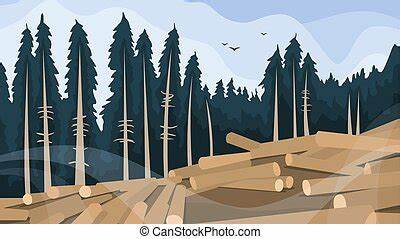
\includegraphics[width=13cm]{figs/logging.jpg}
    \caption{Deforestation.}
    \label{fig:my_label}
\end{figure}

In the traditional view, deforestation is to sacrifice the ecological environment for economic gain. But recent mathematical analysis has led us to a surprising result: proper logging practices can not only improve economic efficiency, but also increase carbon sequestration!
The reason is quite simple: forest products themselves fix part of the carbon, which is basically constant in its service life, and when it reaches its service life, part of the carbon will be returned to the soil by landfill rather than all discharged into the atmosphere. And the land that has been cut down is often replanted with new trees, which also sequester more carbon. Simply put, proper logging strategies can sequester more carbon per unit of land, both in the form of forest products and newly planted trees. That's something you can't do just by using the land for trees.

However, it is important to clarify that we do not support blind overcutting; there is a limit to cutting. We need to find the best balance for trade-offs in time and quantity.

1. Set reasonable rotation period and felling ratio.

2. Set a reasonable proportion of products. Forest products can often be used in a variety of forms to produce a variety of goods, and we can pursue the best strategy by controlling the tree species, location and age of trees harvested.

We recommend that communities further optimize their forest management practices in conjunction with the forest evaluation system, taking into account the ecological, economic, social and sustainability dimensions to achieve a "four best" forest.

Glossary:

Carbon Sequestration: the process of capturing and storing carbon dioxide from the atmosphere.
